\documentclass[a4paper]{article}

\usepackage[english]{babel}
\usepackage[utf8x]{inputenc}
\usepackage{amsmath}
\usepackage{graphicx}
\usepackage[colorinlistoftodos]{todonotes}

\title{CMSC 447 - Artificial Intelligence\\
Project 2 Analysis}
\author{Ying Zhang}
\date{March 18, 2016}

\begin{document}
\maketitle

\section{Introduction}

The goal of Project 2 is to find the local minimum of the function,\\
\(z=\frac{\sin(x^2+3y^2)}{0.1+r^2}+(x^2+5y^2)\times\frac{\exp(1-r^2)}{2}\), \(r=x^2+y^2\), using three local search algorithms, including Hill Climbing, Hill Climbing with Random Restarts, and Simulated Annealing. After the global minimum is found, display the path that they took to find the global minimum on the screen.

\section{Performance}

From the result of the Project 2 execution, Simulated Annealing appears to have the best result among the three local searches. Unlike Hill Climbing and Hill Climbing with Random Restarts, Simulated Annealing's control parameter, T, helps it to avoid becoming trapped at local minimum. Hill Climbing and Hill Climbing with Random Restarts use greedy algorithm, that is they only accept current state as the new state only if it is less than the previous global minimum. Whereas there is still a probability for Simulated Annealing to accept current state as the new state even if it is greater than the previous global minimum. Hill Climbing and Hill Climbing with Random Restarts only explore the areas with values less than its current global minimum, and Simulated Annealing exploits a broader search space with its probability function,\\ \(p(move_A\rightarrow _B) = \exp\frac{f(B)-f(A)}{T}\).\\

\noindent The time for Hill Climbing with Random Restarts to finish execute depends on the number of restart that is assigned during function calls. When Hill Climbing with Random Restarts needs to have numerous restarts, then the running time tend to be longer. Same applies to Simulated Annealing, higher initial temperature will slow down the execution performance.

\section{Results}

\begin{figure}
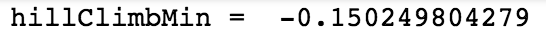
\includegraphics[scale=0.5]{HC.png}
\caption{Global minimum found by Hill Climbing}
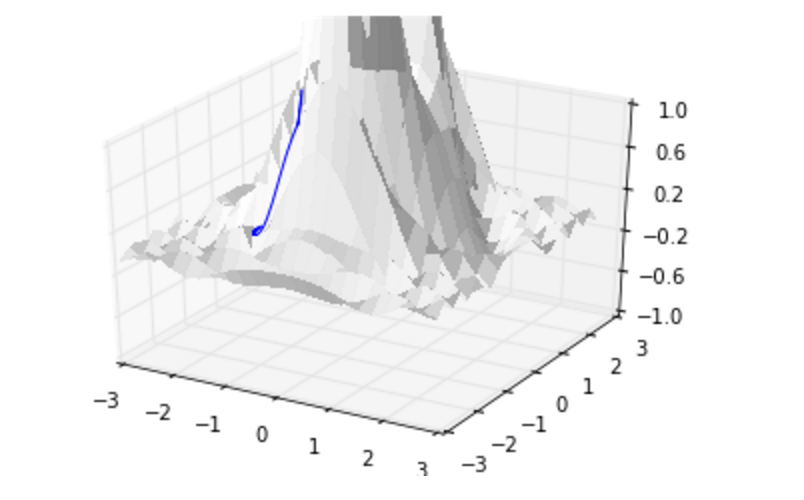
\includegraphics[scale=0.5]{hillClimbing.png}
\caption{Path to global minimum using Hill Climbing}
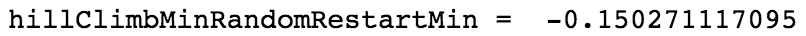
\includegraphics[scale=0.5]{RR.png}
\caption{Global minimum found by Hill Climbing with Random Restarts}
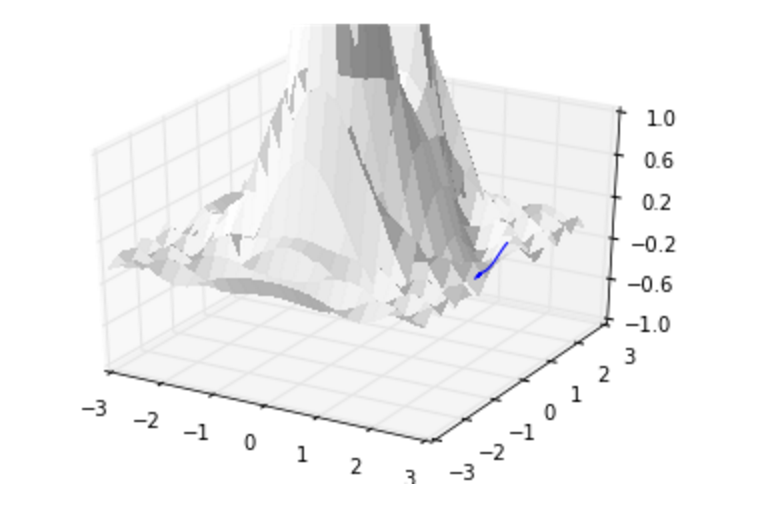
\includegraphics[scale=0.5]{random.png}
\caption{Path to global minimum using Hill Climbing with Random Restarts}
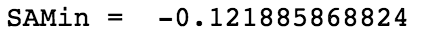
\includegraphics[scale=0.5]{SAM.png}
\caption{Global minimum found by Simulated Annealing}
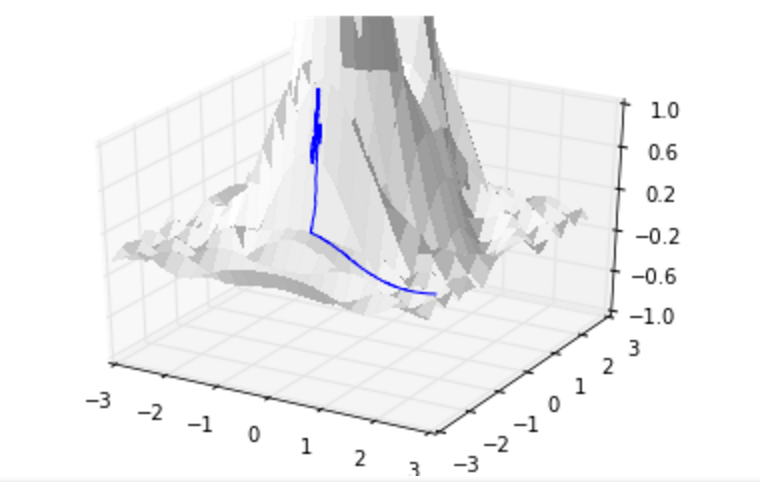
\includegraphics[scale=0.5]{SA.png}
\caption{Path to global minimum using Simulated Annealing}
\end{figure}

\newpage
\section{References}

\begin{enumerate}
\item https://en.wikibooks.org/wiki/LaTeX/Mathematics
\item https://www.overleaf.com
\item https://en.wikibooks.org/wiki/LaTeX/Paragraph\_Formatting\#Paragraph\_indent\_and\_break
\end{enumerate}

\end{document}